Through the previous analysis of different approaches to recommendation systems it was recognized that it was needed to do a variation of the hybrid recommendation model, the hybrid model being a combination of the content-based and collaborative forms of recommendation. It was decided to approach it very departmentalized. This means the two methods will not directly interfere with each other, which leads to them remaining fairly simple while still getting the benefit of the hybrid model. This however also means the feedback loop will be slightly weaker. With the gained simplicity the slight precision loss from the weaker feedback loop is, at least for this projects prototype, worth it.

The algorithm ended up being split into three main steps. See Figure \ref{GenRecAlgo}:
\begin{itemize}
	\item Collaborative filtering
	\item Content-based filtering
	\item Merge
\end{itemize}

We will go more into detail about the mechanics of the collaborative and content-based filtering algorithms in the following part of this section. The basic idea of this structure is that the two filtering algorithms each pick a list of the best suited media recommendations for the selected user, based on some kind of weight or coefficient. Then in the merge part the two lists is merged into one list, creating a more precise list than the two recommendation forms could do on their own.

\begin{figure}[H]
\centering
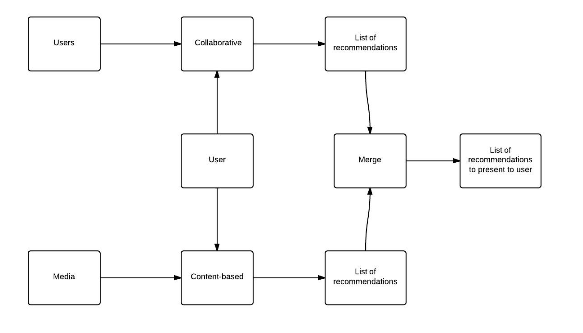
\includegraphics[width=1\textwidth]{Images/RecommendationAlgo.png}
\caption{The general structure of the recommenendation algorithm}
\label{GenRecAlgo}
\end{figure}

\subsection{Collaborative Design}
\label{CollaborativeDes}
\relinput{CollaborativeDes}

\subsection{Content-Based Design}
\label{ContentBasedDes}
\relinput{ContentDes}